\documentclass[11pt,a4paper]{article}

%==============================================================
% PACKAGES
%==============================================================
% --- Encoding and language ---
\usepackage[utf8]{inputenc}
\usepackage[T1]{fontenc}
\usepackage{lmodern}
\usepackage[english]{babel}
\usepackage{microtype}
\usepackage{textgreek}
\usepackage{physics}
\newcommand{\dt}[1]{\dot{#1}}
\newcommand{\ddt}[1]{\ddot{#1}}

% --- Layout ---
\usepackage[margin=2.3cm,top=2.2cm,bottom=2.2cm]{geometry}
\setlength{\headheight}{14pt}
\usepackage{fancyhdr}
\usepackage{enumitem}
\usepackage{mdframed}      % caja gris para los enunciados de las preguntas
\usepackage{titlesec}
\titlespacing*{\section}{0pt}{1.2ex plus 0.2ex minus 0.1ex}{0.5ex plus 0.1ex minus 0.1ex}
\titlespacing*{\subsection}{0pt}{0.9ex plus 0.2ex minus 0.1ex}{0.3ex plus 0.1ex minus 0.1ex}

% --- Spacing around equations ---
\setlength{\abovedisplayskip}{5pt plus 1pt minus 1pt}
\setlength{\belowdisplayskip}{5pt plus 1pt minus 1pt}
\setlength{\abovedisplayshortskip}{2pt plus 1pt minus 1pt}
\setlength{\belowdisplayshortskip}{2pt plus 1pt minus 1pt}

% --- Mathematics and units ---
\usepackage{amsmath, amssymb, amsfonts}
\usepackage{bm}
\usepackage{siunitx}
\sisetup{per-mode=symbol}
\newcommand{\er}{\bm{e}_r}
\newcommand{\ephi}{\bm{e}_\varphi}
\newcommand{\ii}{\bm{i}}
\newcommand{\jj}{\bm{j}}
\newcommand{\kk}{\bm{k}}

% --- Figures and tables ---
\usepackage{graphicx}
\usepackage{epstopdf}      % permite incluir .eps (las figuras de Matlab se guardan como .eps)
\usepackage{xcolor}
\usepackage{caption}
\usepackage{subcaption}
\usepackage{booktabs}
\usepackage{float}
\usepackage{tikz}          % esquema del aro
\graphicspath{{figures/}{figs/}}

% --- Matlab code listings ---
\usepackage{listings}
\lstset{
  language=Matlab,
  basicstyle=\ttfamily\footnotesize,
  keywordstyle=\color{blue},
  commentstyle=\color{green!50!black},
  numbers=left,
  numberstyle=\tiny,
  frame=single,
  breaklines=true
}

% --- Links and cross-references (cargar al final) ---
\usepackage[hidelinks]{hyperref}
\usepackage[capitalise,noabbrev]{cleveref}

%==============================================================
% DOCUMENT DATA  (editar solo aqui)
%==============================================================
\newcommand{\labnumber}{2}
\newcommand{\labgroup}{LA}   % LA o LB

\title{Particle on Oscillating Loop}
\author{Aimar Álvarez Iglesias \and
        Héctor Gonzalez Rodriguez \and
        Santiago Hernández Bejarano}
\date{\today}

%==============================================================
% STYLE
%==============================================================
% --- Header / footer ---
\pagestyle{fancy}
\fancyhf{}
\lhead{Mechanics Applied to Aerospace Engineering}
\rhead{Lab \labnumber{} -- Group \labgroup}
\cfoot{\thepage}
\renewcommand{\headrulewidth}{0.4pt}

% --- Abstract compacto (para que abstract + indice quepan en una pagina) ---
\renewenvironment{abstract}{%
  \begin{center}\bfseries\small\abstractname\end{center}%
  \vspace{-1em}\begin{quotation}\footnotesize}{%
  \end{quotation}\vspace{0.5em}}

% --- Los enunciados de las preguntas se escriben con el entorno estandar
%     "quote", que aqui se redefine como caja gris. ---
\renewenvironment{quote}{%
  \par\medskip
  \begin{mdframed}[backgroundcolor=gray!12, hidealllines=true,
    innerleftmargin=8pt, innerrightmargin=8pt,
    innertopmargin=6pt, innerbottommargin=6pt]\small\itshape\emergencystretch=3em}{%
  \end{mdframed}\par\medskip}

% --- Portada: se redefine \maketitle ---
\makeatletter
\renewcommand{\maketitle}{%
  \begin{titlepage}
    \centering
    \vspace*{0.2cm}

    \IfFileExists{logo_uc3m.png}{%
      
\includegraphics[width=0.30\textwidth]{logo_uc3m.png}\par
      \vspace{0.8cm}
    }{\vspace{1.5cm}}

    {\Large\bfseries Universidad Carlos III de Madrid\par}
    \vspace{0.25cm}
    {\large Aerospace Engineering\par}

    \vspace{1.2cm}

    \noindent\rule{\linewidth}{0.5pt}\par
    \vspace{0.4cm}
    {\huge\bfseries Computer Laboratory Report \labnumber\par}
    \vspace{0.35cm}
    {\LARGE \@title\par}
    \vspace{0.4cm}
    \noindent\rule{\linewidth}{0.5pt}\par

    \vspace{1.0cm}

    {\large Mechanics Applied to Aerospace Engineering\par}
    \vspace{0.25cm}
    {\large Laboratory Group \labgroup\par}

    \vspace{1.0cm}

    {\large\bfseries Authors\par}
    \vspace{0.3cm}
    {\large\def\and{\\}\renewcommand{\arraystretch}{1.3}%
     \begin{tabular}{c}\@author\end{tabular}\par}

    \vfill

    {\large \@date\par}
    \vspace*{0.2cm}
  \end{titlepage}}
\makeatother

%==============================================================
\begin{document}
%==============================================================

\maketitle

\tableofcontents
\vspace{1em}

%==============================================================
\section{Introduction}
In this laboratory the motion of a heavy particle $P$ of mass $m$ that slides without friction on a circular wire of centre $C$ and radius $R$ is studied. The wire lies on a vertical plane $Oxy$, and this plane turns about the vertical axis $Oy$ with the prescribed angular velocity $\bm\Omega(t)=A\omega\sin(\omega t)\,\jj$, where $A$ and $\omega$ are known positive constants. The position of $P$ on the wire is given by the angle $\varphi$ between the axis $Ox$ and the vector $\overrightarrow{CP}$ \cite{guidelines}.

The aim is to write the equation of motion of $P$ in the rotating frame, integrate it with \texttt{ode45}, and use the results to explain the forces of the wire, the energy, the trajectory seen from a fixed frame, when $P$ goes over the top of a fixed loop, and how good the linearized equation is.

\Cref{sec:method} derives the model and explains the numerical setup. \Cref{sec:results} discusses the result of each simulation next to its figure, \cref{sec:discussion} gathers the points that apply to the whole model, and \cref{sec:conclusions} sums up.

%==============================================================
\section{Methodology}\label{sec:method}
\subsection{Kinematics and degree of freedom}
\begin{figure}[htbp]
\centering
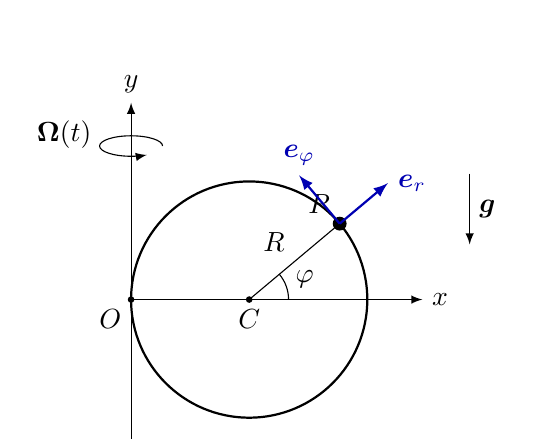
\begin{tikzpicture}[scale=1.0,>=latex]
\def\R{1.5}\def\ph{40}
\pgfmathsetmacro{\px}{\R+\R*cos(\ph)}\pgfmathsetmacro{\py}{\R*sin(\ph)}
\draw[thick] (\R,0) circle (\R);
\draw[->] (0,0) -- (3.7,0) node[right] {$x$};
\draw[->] (0,-1.9) -- (0,2.5) node[above] {$y$};
\fill (0,0) circle (1.2pt) node[below left] {$O$};
\fill (\R,0) circle (1.2pt) node[below] {$C$};
\draw (\R,0) -- (\px,\py) node[midway,above left] {$R$};
\fill (\px,\py) circle (2.5pt) node[above left] {$P$};
\draw (\R+0.5,0) arc (0:\ph:0.5); \node at ({\R+0.75*cos(\ph/2)},{0.75*sin(\ph/2)}) {$\varphi$};
\draw[->,thick,blue!70!black] (\px,\py) -- ++({0.8*cos(\ph)},{0.8*sin(\ph)}) node[right] {$\er$};
\draw[->,thick,blue!70!black] (\px,\py) -- ++({-0.8*sin(\ph)},{0.8*cos(\ph)}) node[above] {$\ephi$};
\draw[->] (0.4,1.95) arc (0:300:0.4 and 0.13); \node at (-0.85,2.1) {$\bm\Omega(t)$};
\draw[->] (4.3,1.6) -- (4.3,0.7) node[midway,right] {$\bm g$};
\end{tikzpicture}
\caption{Geometry of the problem. The plane $Oxy$ turns about $Oy$; $\kk=\ii\times\jj$ points out of the page. The polar basis $\{\er,\ephi\}$ is attached to $P$.}\label{fig:geom}
\end{figure}
Two reference frames are used. $Oxyz$ moves with the plane of the wire: $\ii$ lies along the horizontal diameter, $\jj$ points upwards along the axis and $\kk=\ii\times\jj$ is normal to the plane. $Ox_1y_1z_1$ is fixed and coincides with $Oxyz$ at $t=0$. From the figure, the axis $Oy$ is tangent to the wire at $O$, so $\overrightarrow{OC}=R\,\ii$ (\cref{fig:geom}).

\textbf{Degree of freedom.} A free particle has three coordinates. The wire adds two constraints: $P$ must stay in the plane $Oxy$ and at a distance $R$ from $C$. This leaves $3-2=1$ degree of freedom, parametrised by $\varphi$. The plane turns with a known law, so the position in the fixed frame depends on $\varphi$ and also explicitly on $t$.

\textbf{Motion of the plane.} The angle $\theta$ turned by the plane satisfies $\dt\theta=\Omega$ with $\theta(0)=0$. With the change $u=\omega\tau$, $\dd u=\omega\,\dd\tau$, and Barrow's rule,
\begin{equation}
\theta(t)=\int_0^t A\omega\sin(\omega\tau)\,\dd\tau=A\int_0^{\omega t}\sin u\,\dd u=A\big[-\cos u\big]_0^{\omega t}=A\big(1-\cos\omega t\big).
\label{eq:theta}
\end{equation}
So the plane swings between $\theta=0$ and $\theta=2A$; with $A=\pi$ it makes a full turn in $T/2$ and comes back, where $T=2\pi/\omega$. A rotation of angle $\theta$ about the vertical axis relates both bases: the columns of
\begin{equation}
[{}_1R_0]=\begin{pmatrix}\cos\theta&0&\sin\theta\\0&1&0\\-\sin\theta&0&\cos\theta\end{pmatrix}
\label{eq:rot}
\end{equation}
are the components of $\ii$, $\jj$, $\kk$ in $\{\ii_1,\jj_1,\kk_1\}$. The columns are orthonormal, so $[{}_1R_0][{}_1R_0]^T=I$, and $\det[{}_1R_0]=\cos^2\theta+\sin^2\theta=1$. As a check, $\ii=\cos\theta\,\ii_1-\sin\theta\,\kk_1$ gives $\dd\ii/\dd t=-\dt\theta(\sin\theta\,\ii_1+\cos\theta\,\kk_1)=-\Omega\,\kk=\bm\Omega\times\ii$.

\textbf{Relative motion.} Let $\er=\cos\varphi\,\ii+\sin\varphi\,\jj$ and $\ephi=-\sin\varphi\,\ii+\cos\varphi\,\jj$. The position of $P$ is
\begin{equation}
\bm r=\overrightarrow{OC}+\overrightarrow{CP}=R(1+\cos\varphi)\,\ii+R\sin\varphi\,\jj,\qquad x\equiv R(1+\cos\varphi),
\label{eq:pos}
\end{equation}
where $x$ is the distance from $P$ to the axis. Differentiating each component in $Oxyz$ with the chain rule, $\frac{\dd}{\dd t}[R(1+\cos\varphi)]=-R\dt\varphi\sin\varphi$ and $\frac{\dd}{\dd t}[R\sin\varphi]=R\dt\varphi\cos\varphi$, so
\begin{equation}
\bm v_{\text{rel}}=-R\dt\varphi\sin\varphi\,\ii+R\dt\varphi\cos\varphi\,\jj=R\dt\varphi\,\ephi .
\label{eq:vrel}
\end{equation}
With the product rule, $\frac{\dd}{\dd t}(-R\dt\varphi\sin\varphi)=-R(\ddt\varphi\sin\varphi+\dt\varphi^2\cos\varphi)$ and $\frac{\dd}{\dd t}(R\dt\varphi\cos\varphi)=R(\ddt\varphi\cos\varphi-\dt\varphi^2\sin\varphi)$:
\begin{equation}
\bm a_{\text{rel}}=-R(\ddt\varphi\sin\varphi+\dt\varphi^2\cos\varphi)\,\ii+R(\ddt\varphi\cos\varphi-\dt\varphi^2\sin\varphi)\,\jj=R\ddt\varphi\,\ephi-R\dt\varphi^2\,\er .
\label{eq:arel}
\end{equation}

\textbf{Absolute motion.} $O$ is on the axis and does not move, so $\bm v=\bm v_{\text{rel}}+\bm\Omega\times\bm r$ and $\bm a=\bm a_{\text{rel}}+\dt{\bm\Omega}\times\bm r+\bm\Omega\times(\bm\Omega\times\bm r)+2\bm\Omega\times\bm v_{\text{rel}}$, with $\Omega=A\omega\sin\omega t$ and $\dt\Omega=A\omega^2\cos\omega t$. Using $\jj\times\ii=-\kk$, $\jj\times\jj=\bm 0$ and $\jj\times\kk=\ii$, the four products are
\begin{align}
\bm\Omega\times\bm r&=\Omega\,x\,(\jj\times\ii)+\Omega R\sin\varphi\,(\jj\times\jj)=-\Omega x\,\kk,\qquad
\dt{\bm\Omega}\times\bm r=-\dt\Omega x\,\kk,\label{eq:prod1}\\
\bm\Omega\times(\bm\Omega\times\bm r)&=\Omega\,\jj\times(-\Omega x\,\kk)=-\Omega^2x\,(\jj\times\kk)=-\Omega^2x\,\ii,\label{eq:prod2}\\
2\bm\Omega\times\bm v_{\text{rel}}&=2\Omega R\dt\varphi\big[-\sin\varphi\,(\jj\times\ii)+\cos\varphi\,(\jj\times\jj)\big]=2\Omega R\dt\varphi\sin\varphi\,\kk .\label{eq:prod3}
\end{align}
Adding them,
\begin{align}
\bm v&=R\dt\varphi\,\ephi-\Omega x\,\kk,\label{eq:vel}\\
\bm a&=\big[-R(\ddt\varphi\sin\varphi+\dt\varphi^2\cos\varphi)-\Omega^2x\big]\ii+R(\ddt\varphi\cos\varphi-\dt\varphi^2\sin\varphi)\,\jj+\big[-\dt\Omega x+2\Omega R\dt\varphi\sin\varphi\big]\kk .\label{eq:acc}
\end{align}
Since $\ephi\perp\kk$, the speed is $|\bm v|^2=R^2\dt\varphi^2+\Omega^2x^2$.

\subsection{Forces and equation of motion}
Two real forces act on $P$: its weight and the reaction of the wire. The wire is smooth, so the reaction has no component along the tangent $\ephi$:
\begin{equation}
\bm W=-mg\,\jj=-mg\sin\varphi\,\er-mg\cos\varphi\,\ephi,\qquad \bm N=N_r\,\er+N_z\,\kk ,
\label{eq:forces}
\end{equation}
where $\jj=\sin\varphi\,\er+\cos\varphi\,\ephi$ was used. In the rotating frame the inertia forces have to be added. From \cref{eq:prod1,eq:prod2,eq:prod3},
\begin{align}
\bm F_{\text{cf}}&=-m\bm\Omega\times(\bm\Omega\times\bm r)=m\Omega^2x\,\ii=mA^2\omega^2R\sin^2(\omega t)(1+\cos\varphi)\big[\cos\varphi\,\er-\sin\varphi\,\ephi\big],\label{eq:Fcf}\\
\bm F_{\text{Eul}}&=-m\dt{\bm\Omega}\times\bm r=m\dt\Omega x\,\kk=mA\omega^2R\cos(\omega t)(1+\cos\varphi)\,\kk,\label{eq:Feul}\\
\bm F_{\text{Cor}}&=-2m\bm\Omega\times\bm v_{\text{rel}}=-2m\Omega R\dt\varphi\sin\varphi\,\kk=-2mA\omega R\dt\varphi\sin(\omega t)\sin\varphi\,\kk ,\label{eq:Fcor}
\end{align}
with $\ii=\cos\varphi\,\er-\sin\varphi\,\ephi$. Newton's second law in $Oxyz$ reads $m\bm a_{\text{rel}}=\bm W+\bm N+\bm F_{\text{cf}}+\bm F_{\text{Eul}}+\bm F_{\text{Cor}}$. The tangent $\ephi$ is the only direction free of the unknown reaction, and the Euler and Coriolis forces point along $\kk$, so projecting on $\ephi$ gives $mR\ddt\varphi=-mg\cos\varphi-m\Omega^2x\sin\varphi$, that is
\begin{equation}
\ddt\varphi=-\frac{g}{R}\cos\varphi-A^2\omega^2\sin^2(\omega t)\,(1+\cos\varphi)\sin\varphi .
\label{eq:eom}
\end{equation}
The other two projections give the reaction. Along $\er$, $-mR\dt\varphi^2=N_r-mg\sin\varphi+m\Omega^2x\cos\varphi$, and along $\kk$, $0=N_z+m\dt\Omega x-2m\Omega R\dt\varphi\sin\varphi$:
\begin{align}
N_r&=-mR\dt\varphi^2+mg\sin\varphi-mA^2\omega^2R\sin^2(\omega t)(1+\cos\varphi)\cos\varphi ,\label{eq:Nr}\\
N_z&=mA\omega R\big[2\dt\varphi\sin(\omega t)\sin\varphi-\omega\cos(\omega t)(1+\cos\varphi)\big].\label{eq:Nz}
\end{align}
The meaning of each term in \cref{eq:eom} is the following:
\begin{itemize}[noitemsep,topsep=2pt]
\item If the plane does not turn ($A=0$), the equation is the one of a pendulum, $\ddt\varphi=-(g/R)\cos\varphi$, with $\varphi$ measured from the horizontal. The bottom, $\varphi=-\pi/2$, is a stable equilibrium and the top, $\varphi=\pi/2$, an unstable one.
\item Only the centrifugal force enters the equation, because it is the only inertia force in the plane of the wire. The Euler and Coriolis forces are normal to the plane and only load the wire through $N_z$.
\item The centrifugal term is at most $(A\omega)^2/(g/R)=\pi^2\cdot0.01/9.81\approx1\%$ of the gravity term for the data of item 5, so the rotation is a weak perturbation of the pendulum.
\item The wire holds $P$ on both sides, so $\bm N$ can take any sign. Unlike the string of Lab~1, there is no condition that stops the model.
\end{itemize}

\subsection{Mechanical energy}
With the absolute velocity of \cref{eq:vel}, the kinetic and gravitational potential energies are
\begin{equation}
E_k=\tfrac12m\big(R^2\dt\varphi^2+\Omega^2x^2\big),\qquad E_p=mgR\sin\varphi,\qquad E=E_k+E_p .
\label{eq:E}
\end{equation}
In the fixed frame the weight is included in $E$, so $\dd E/\dd t$ is the power of the reaction. Using \cref{eq:forces,eq:vel} and $\er\cdot\ephi=0$,
\begin{equation}
\frac{\dd E}{\dd t}=\bm N\cdot\bm v=\big(N_r\,\er+N_z\,\kk\big)\cdot\big(R\dt\varphi\,\ephi-\Omega x\,\kk\big)=-\Omega\,x\,N_z .
\label{eq:Edot}
\end{equation}
The wire moves with the plane and pushes $P$ along $\kk$, so it does work whenever $\Omega\neq0$: $E$ is conserved only for $A=0$.

\subsection{Fixed loop: condition to go over the top}\label{sec:crit}
For $A=0$, multiplying \cref{eq:eom} by $\dt\varphi$ gives $\dt\varphi\ddt\varphi+(g/R)\cos\varphi\,\dt\varphi=0$. By the chain rule, $\frac{\dd}{\dd t}(\tfrac12\dt\varphi^2)=\dt\varphi\ddt\varphi$ and $\frac{\dd}{\dd t}\sin\varphi=\cos\varphi\,\dt\varphi$, so
\begin{equation}
\frac{\dd}{\dd t}\Big[\tfrac12\dt\varphi^2+\frac gR\sin\varphi\Big]=0\quad\Rightarrow\quad \tfrac12\dt\varphi^2+\frac gR\sin\varphi=\tfrac12\dt\varphi_0^2+\frac gR\sin\varphi_0 ,
\label{eq:first}
\end{equation}
which is $E/(mR^2)$ = constant. The potential energy is largest at the top, $\varphi=\pi/2$, where $E_p=mgR$. If $P$ reaches the top with $\dt\varphi\neq0$ it goes over it and $\varphi$ keeps growing; otherwise it stops before and comes back. Setting $\dt\varphi^2>0$ at $\varphi=\pi/2$ in \cref{eq:first} gives the criterion
\begin{equation}
|\dt\varphi_0|>\dt\varphi_c=\sqrt{\frac{2g}{R}\big(1-\sin\varphi_0\big)} .
\label{eq:crit}
\end{equation}
The equality defines the separatrix $\dt\varphi=\pm\sqrt{(2g/R)(1-\sin\varphi)}$, along which $P$ approaches the top but needs an infinite time to reach it. Below it, $\varphi$ oscillates between the two angles where $\dt\varphi=0$, that is, $\sin\varphi=\sin\varphi_0+R\dt\varphi_0^2/(2g)$. \Cref{tab:crit} applies the criterion to the nine initial conditions of item 7.
\begin{table}[htbp]
\centering
\caption{Critical rate of \cref{eq:crit} ($g/R=\SI{9.81}{s^{-2}}$) and predicted motion for the nine initial conditions.}\label{tab:crit}
\begin{tabular}{ccccc}
\toprule
$\varphi_0$ (rad) & $\dt\varphi_c$ (rad/s) & $\dt\varphi_0=0$ & $\dt\varphi_0=1.5$ rad/s & $\dt\varphi_0=3$ rad/s\\
\midrule
$0$ & 4.429 & oscillates & oscillates & oscillates\\
$\pi/4$ & 2.397 & oscillates & oscillates & goes over the top\\
$\pi/2$ & 0 & rest at the top (unstable) & goes over the top & goes over the top\\
\bottomrule
\end{tabular}
\end{table}

\subsection{Linearized equation}\label{sec:lin}
Now $A^2\ll g/(R\omega^2)$ and $\varphi=\delta-\pi/2$ with $|\delta|\ll1$. Then $\cos\varphi=\cos(\delta-\pi/2)=\sin\delta\approx\delta$, $\sin\varphi=-\cos\delta\approx-1$, $1+\cos\varphi\approx1+\delta$ and $\ddt\varphi=\ddt\delta$. Substituting in \cref{eq:eom},
\begin{equation}
\ddt\delta=-\frac gR\,\delta+\Omega^2(1+\delta)=-\frac gR\,\delta+\Omega^2+\Omega^2\delta .
\end{equation}
The hypothesis $A^2\ll g/(R\omega^2)$ means $\Omega^2\le A^2\omega^2\ll g/R$, so the term $\Omega^2\delta$ is small next to $(g/R)\delta$ and is dropped. With $\sin^2(\omega t)=\tfrac12[1-\cos(2\omega t)]$,
\begin{equation}
\ddt\delta+\omega_n^2\,\delta=\Omega^2=F_0\big[1-\cos(2\omega t)\big],\qquad \omega_n=\sqrt{g/R},\qquad F_0=\tfrac12A^2\omega^2 .
\label{eq:lin}
\end{equation}
This is a forced oscillator without damping: natural frequency $\omega_n$ and forcing at $2\omega$ \cite{notes}. The statement gives no initial conditions for item 8, and they are not given in the problem sheet either \cite{problems}. Here $P$ starts at rest at the bottom, $\delta(0)=0$ and $\dt\delta(0)=0$, so all its motion comes from the loop. The particular solution is a constant $F_0/\omega_n^2$ plus $C\cos(2\omega t)$; substituting the second one, $(\omega_n^2-4\omega^2)C=-F_0$. Adding the free solution $a\cos\omega_nt+b\sin\omega_nt$ and imposing the initial conditions ($\dt\delta(0)=b\,\omega_n=0$),
\begin{equation}
\delta(t)=\frac{F_0}{\omega_n^2}-\frac{F_0\cos(2\omega t)}{\omega_n^2-4\omega^2}+\Big(\frac{F_0}{\omega_n^2-4\omega^2}-\frac{F_0}{\omega_n^2}\Big)\cos(\omega_nt),\qquad 2\omega\neq\omega_n .
\label{eq:linsol}
\end{equation}
So $P$ oscillates about $\delta_s=F_0/\omega_n^2=A^2R\omega^2/(2g)$, slightly outwards from the bottom. When $2\omega=\omega_n$ the denominator vanishes. This is resonance, and the particular solution changes to $-\frac{F_0}{2\omega_n}t\sin(\omega_nt)$, which satisfies $\ddt\delta+\omega_n^2\delta=-F_0\cos(\omega_nt)$. With the same initial conditions,
\begin{equation}
\delta(t)=\frac{F_0}{\omega_n^2}\big(1-\cos\omega_nt\big)-\frac{F_0}{2\omega_n}\,t\sin(\omega_nt),\qquad 2\omega=\omega_n ,
\label{eq:res}
\end{equation}
whose amplitude grows linearly with time. Sooner or later $\delta\ll1$ fails, and the linearization with it.

\subsection{Numerical method}
\Cref{eq:eom} is a second order nonlinear equation with time-dependent coefficients. To integrate it with \texttt{ode45} \cite{matlab} it is written as a first order system for the state vector $\bm X=[\varphi,\dt\varphi]^T$:
\begin{equation}
\frac{\dd\bm X}{\dd t}=\begin{pmatrix}X_2\\[2pt] -\dfrac gR\cos X_1-\Omega(t)^2\,(1+\cos X_1)\sin X_1\end{pmatrix},\qquad \bm X(0)=\begin{pmatrix}\varphi_0\\ \dt\varphi_0\end{pmatrix},\qquad \Omega(t)=A\omega\sin(\omega t).
\label{eq:system}
\end{equation}
This system is the MATLAB function \texttt{diffeq(t,X,g,w,R,A)}, and \cref{eq:lin} is \texttt{diffeqlin} with the state $[\delta,\dt\delta]^T$. The tolerances are $10^{-8}$ (relative) and $10^{-10}$ (absolute). In item 5 the solution is stored at \num{10000} instants in $[0,3T]$, about 125 points for each oscillation of $\varphi$, well above the sampling needed to draw it \cite{guidelines}. The forces and energies are then computed from the stored $\varphi$ and $\dt\varphi$ with \cref{eq:Fcf,eq:Feul,eq:Fcor,eq:Nr,eq:Nz,eq:E}. To check \cref{eq:Edot} without adding a state, the work of the wire is computed afterwards from the power $P_i=-\Omega_ix_iN_{z,i}$ with the trapezoidal rule,
\begin{equation}
W_n=\sum_{i=1}^{n-1}\tfrac12\,(P_i+P_{i+1})(t_{i+1}-t_i),
\label{eq:W}
\end{equation}
and compared with $E-E_0$. The position in the fixed frame follows from \cref{eq:theta,eq:rot}: $x_1=x\cos\theta$, $y_1=R\sin\varphi$, $z_1=-x\sin\theta$. In all cases $g=\SI{9.81}{m/s^2}$ and $m=\SI{1}{kg}$; the three simulations are listed in \cref{tab:sims}.
\begin{table}[htbp]
\centering
\caption{Simulations. In item 8, $\omega_n=\sqrt{g/R}=\SI{31.32}{rad/s}$.}\label{tab:sims}
\small
\begin{tabular}{llcccp{5.4cm}}
\toprule
Item & Case & $A$ (rad) & $R$ (m) & $\omega$ (rad/s) & Initial conditions and time\\
\midrule
5, 6 & oscillating loop & $\pi$ & 1 & 0.1 & $\varphi_0=0$, $\dt\varphi_0=0$; $t\in[0,3T]$, $T=\SI{62.83}{s}$\\
7 & fixed loop & 0 & 1 & -- & \cref{tab:crit}, and $\varphi_0=\pi/4$, $\dt\varphi_0=(1\pm0.01)\,\dt\varphi_c$; $t\in[0,4]$ s\\
8 & linearization & 0.1 & 0.01 & $\omega_n$, $\omega_n/2$, $\omega_n/4$ & $\delta_0=0$, $\dt\delta_0=0$; $t\in[0,10]$ s\\
\bottomrule
\end{tabular}
\end{table}

%==============================================================
\section{Results}\label{sec:results}
\subsection{Oscillating loop: angle, reaction and inertia forces}
At $t=0$ the loop is at rest ($\Omega(0)=0$) and \cref{eq:eom} gives $\ddt\varphi(0)=-g/R=\SI{-9.81}{rad/s^2}$, the value printed by the code. $P$ falls from the end of the horizontal diameter and swings between $\varphi=0$ and $\varphi=-\pi$ (\cref{fig:loop}a,b). At $\varphi=-\pi$ it is at $O$, on the axis. The period is \SI{2.37}{s}, longer than $2\pi\sqrt{R/g}=\SI{2.006}{s}$ because the amplitude about the bottom is $90^\circ$ and the small-oscillation result does not apply. The amplitude does not change over the three periods of the loop: the centrifugal term is only 1\% of gravity. The largest angle is $\varphi=\SI{0.0118}{rad}$, so the energy given by the wire lifts $P$ about \SI{1}{cm} above its starting height.

The radial reaction (\cref{fig:loop}c) goes from 0 at the turning points to \SI{-29.43}{N} at the bottom. Its value is $-3mg$: at the bottom \cref{eq:first} gives $\dt\varphi^2=2g/R$, and \cref{eq:Nr} gives $N_r=-2mg-mg$. The sign is negative because the wire has to pull $P$ towards $C$ to give it the centripetal acceleration. The normal reaction (\cref{fig:loop}d) reaches $\pm\SI{2.78}{N}$. Almost all of it balances the Coriolis force (\cref{fig:loop}f), which is $2mA\omega R\dt\varphi_{\max}=2\pi(0.1)(4.43)=\SI{2.78}{N}$ at most. It is large because $P$ moves fast along the wire ($\dt\varphi$ up to \SI{4.4}{rad/s}) while the plane turns. Its envelope follows $|\sin\omega t|$ and almost vanishes at $t=0,\,T/2,\,T,\dots$, when the plane stops to reverse and only the small Euler term is left. The centrifugal force (\cref{fig:loop}e) is always positive, pointing away from the axis, and peaks at $m(A\omega)^2(2R)=\SI{0.197}{N}$ at $t=T/4,\,3T/4,\dots$, when $\Omega^2$ is largest. The Euler force follows $\cos\omega t$ and stays below \SI{0.063}{N}, because the loop changes its rate slowly: $|\dt\Omega|\le A\omega^2=\SI{0.031}{rad/s^2}$.

\begin{figure}[!htb]
\centering
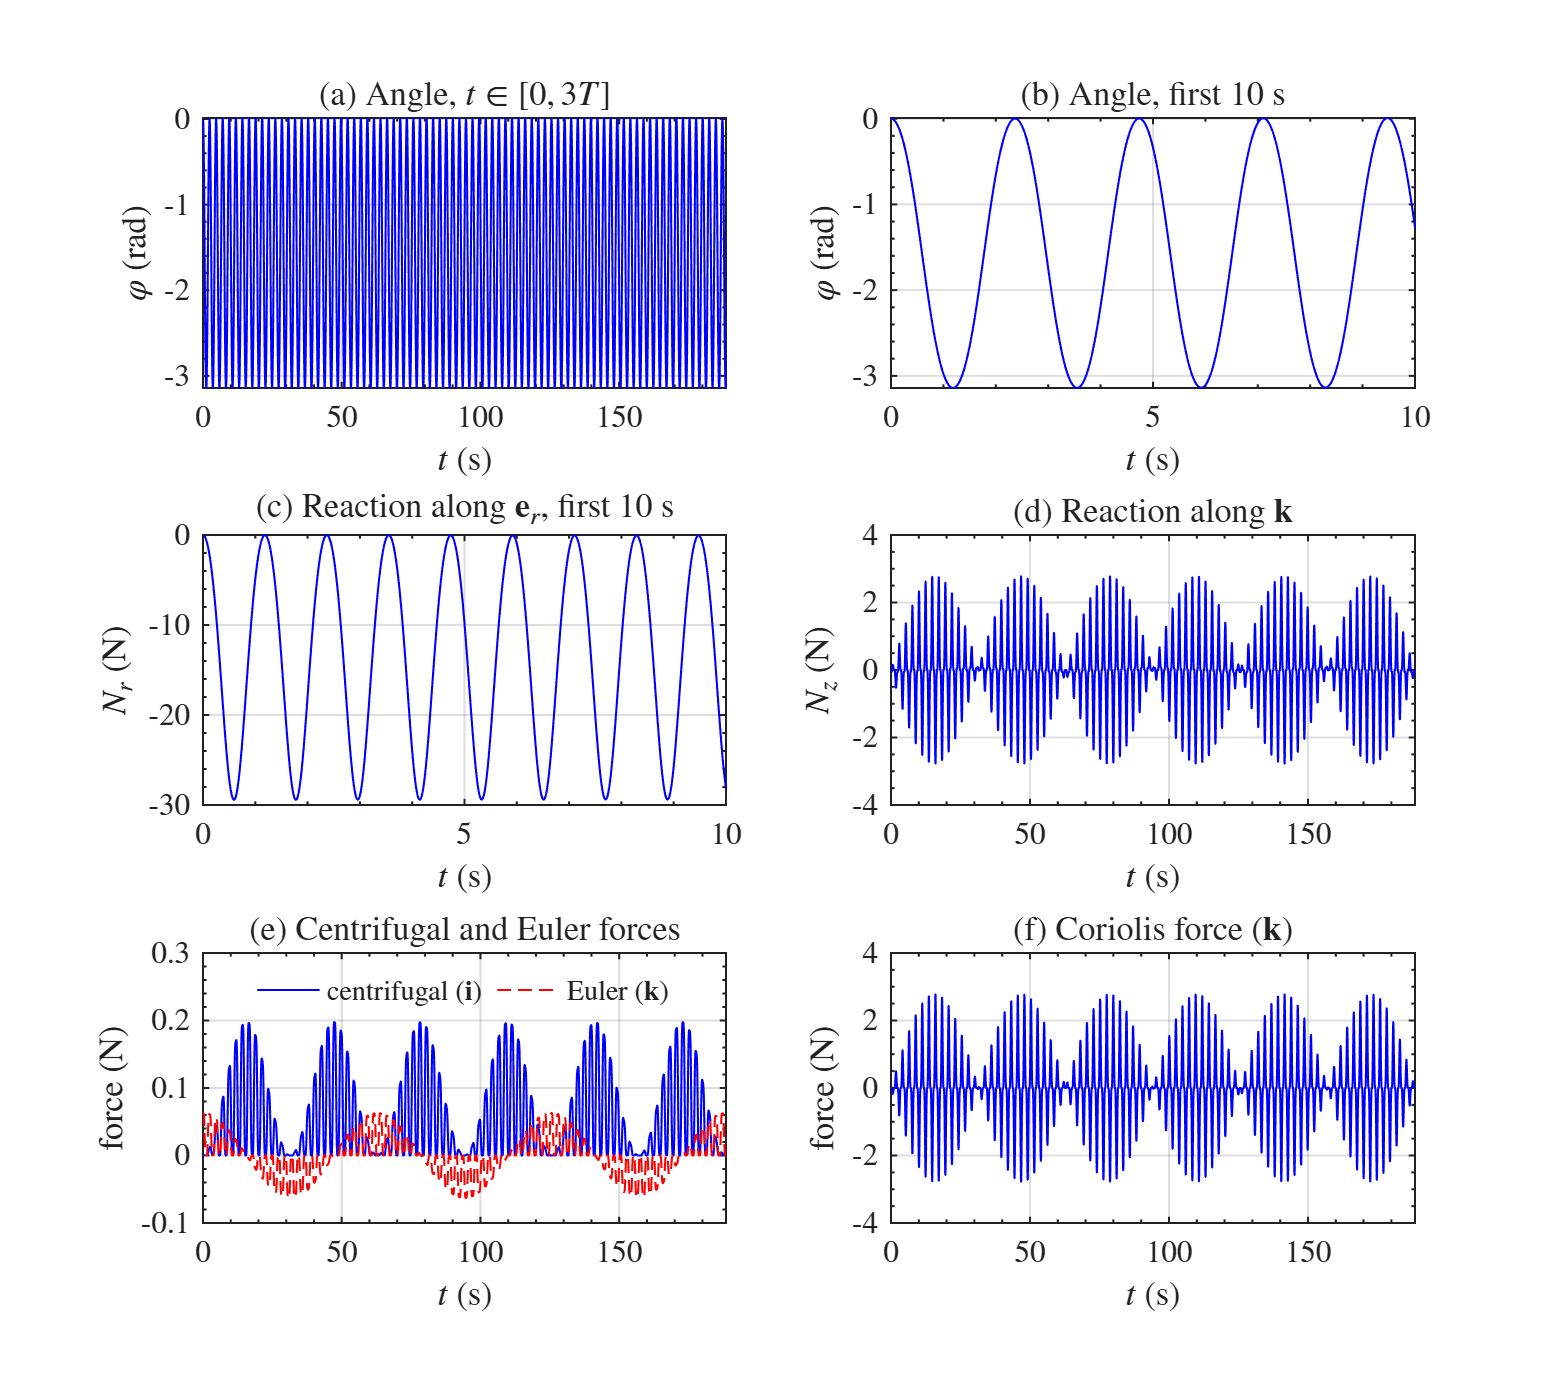
\includegraphics[width=0.76\textwidth]{Fig_2.png}
\caption{Oscillating loop, item 5. (a) Angle in $[0,3T]$ and (b) in the first \SI{10}{s}. (c) Reaction along $\er$, first \SI{10}{s}. (d) Reaction along $\kk$. (e) Centrifugal ($\ii$) and Euler ($\kk$) forces. (f) Coriolis force ($\kk$).}\label{fig:loop}
\end{figure}

\subsection{Energy}
$E_k$ and $E_p$ exchange about \SI{9.8}{J} in every oscillation (\cref{fig:energy}a), as in a pendulum. Their sum is not constant (\cref{fig:energy}b): $E-E_0$ moves between \SI{-0.082}{J} and \SI{0.313}{J}, with a fast oscillation at the frequency of $\varphi$ inside an envelope that follows $\Omega^2$. While $|\Omega|$ grows, the wire pushes $P$ along the direction in which the plane moves and gives it energy, and while $|\Omega|$ decreases it takes the energy back. The loop changes its rate slowly compared with the oscillation ($T=\SI{62.8}{s}$ against \SI{2.37}{s}), so the energy returns to $E_0$ every time the plane stops, and after $3T$ the net gain is only \SI{0.0006}{J}. This also explains why the amplitude of $\varphi$ in \cref{fig:loop}a does not drift.

The work of the wire from \cref{eq:W} lies on top of $E-E_0$; the largest difference is \SI{1.5e-4}{J}, 0.05\% of the range of $E$, and comes from the trapezoidal rule on the stored points. This confirms \cref{eq:Edot} and the expressions of $N_z$ and $E$ used in the code. Repeating the integration with tolerances $10^{-11}$ and $10^{-12}$ changes $\varphi$ by at most \SI{1.4e-4}{rad}.

\begin{figure}[!htb]
\centering
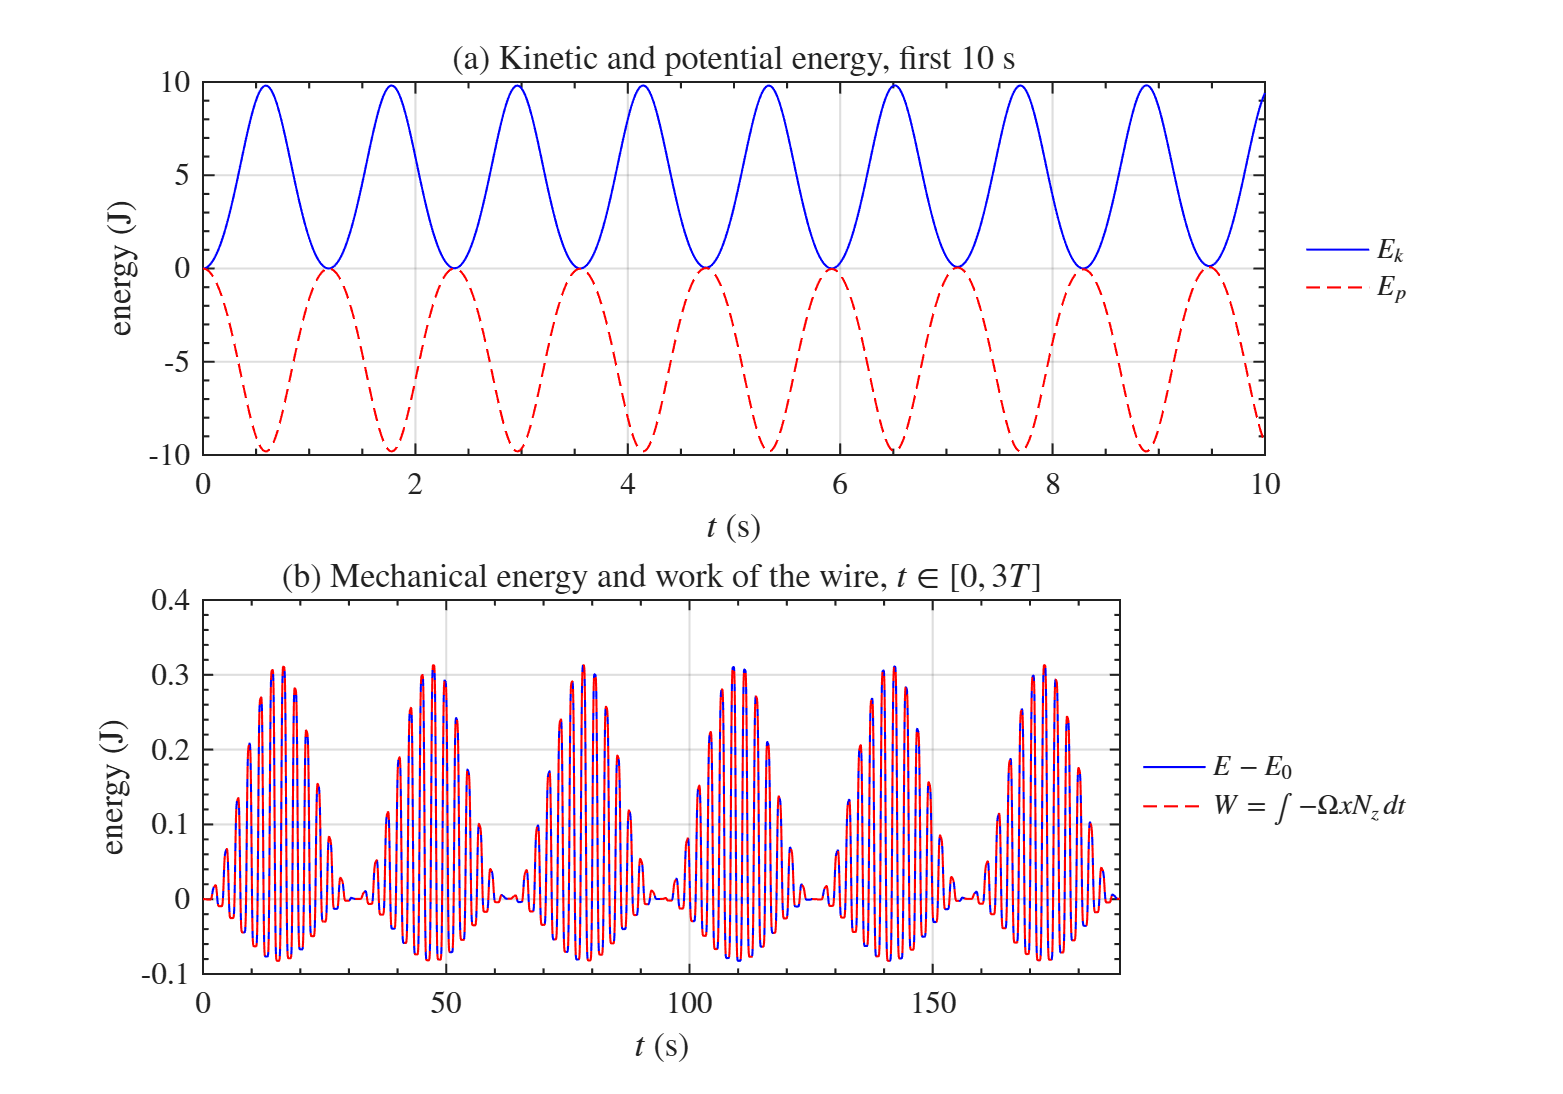
\includegraphics[width=0.68\textwidth]{Fig_3.png}
\caption{Energy, item 5. (a) Kinetic and potential energy in the first \SI{10}{s}; the same pattern repeats over the whole interval. (b) Increment of mechanical energy and work of the wire, \cref{eq:W}, in $[0,3T]$.}\label{fig:energy}
\end{figure}

\subsection{Trajectory in the fixed frame}
$P$ always stays on the surface obtained by turning the circle about $Oy$, a torus whose hole has closed because the circle touches the axis at $O$ (\cref{fig:traj}a). Seen from above (\cref{fig:traj}b), each oscillation of $\varphi$ draws one petal: $P$ goes out to $x=2R$ when $\varphi=0$ and back to the axis when $\varphi=-\pi$. The petals spread around the axis because the plane turns from $\theta=0$ to $\theta=2\pi$ at $t=T/2$ and back to 0 at $t=T$ (\cref{eq:theta}). The three periods draw almost the same curve; they are not identical because the period of $\varphi$ (\SI{2.37}{s}) does not divide $T$. As a check, $\sqrt{x_1^2+z_1^2}$ equals $x$ to \SI{2e-16}{m}, since the rotation in \cref{eq:rot} does not change the distance to the axis.

The script also writes an animation of the first period, \texttt{trajectory\_P.avi}, which is included in the submitted folder. For each frame the wire is drawn turned by $\theta(t_k)$, together with the axis, the trail of $P$ up to $t_k$ and the particle. One frame is taken every 6 stored points, about 20 frames for each oscillation of $\varphi$, so the motion is not undersampled; this gives 556 frames, played at 30 frames per second. The guidelines suggest \texttt{getframe} \cite{guidelines}, but when the code was run without a screen it sometimes returned frames of different sizes, which \texttt{VideoWriter} rejects. Each frame is therefore printed to a fixed $560\times480$ image with \texttt{print(gcf,'-RGBImage','-r80')} and added to the video with \texttt{writeVideo}.

\begin{figure}[!htb]
\centering
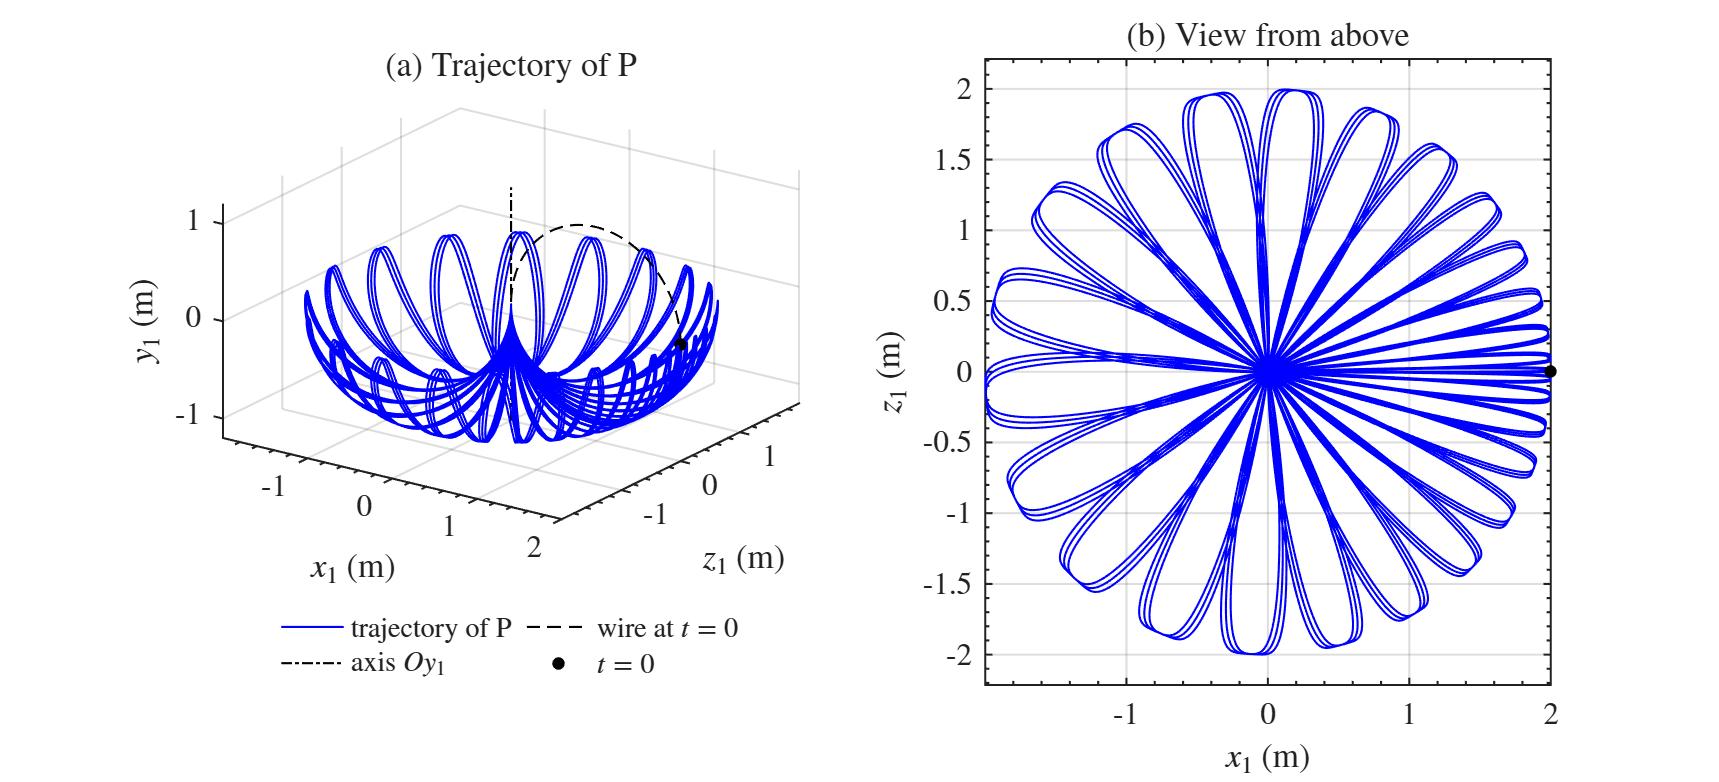
\includegraphics[width=0.82\textwidth]{Fig_4.png}
\caption{Trajectory of $P$ in the fixed frame $Ox_1y_1z_1$ for $t\in[0,3T]$. (a) Three-dimensional view with the wire at $t=0$ and the axis of rotation. (b) View from above.}\label{fig:traj}
\end{figure}

\subsection{Fixed loop: phase portrait}
\Cref{fig:phase}a shows the nine cases of \cref{tab:crit} with the separatrix of \cref{eq:crit}. Five cases, $(0,0)$, $(0,1.5)$, $(0,3)$, $(\pi/4,0)$ and $(\pi/4,1.5)$, give closed curves around the stable equilibrium $(-\pi/2,0)$: $\varphi$ oscillates, as predicted. Their periods grow from \SI{2.37}{s} to \SI{3.36}{s} as the curve gets closer to the separatrix, because $P$ moves slowly near the top. The cases $(\pi/4,3)$, $(\pi/2,1.5)$ and $(\pi/2,3)$ start above the separatrix and give open curves: $\varphi$ increases steadily, with the lowest $\dt\varphi$ at the top and the highest at the bottom of each turn. The case $(\pi/2,0)$ is the unstable equilibrium and stays as a point; numerically $\cos(\pi/2)\approx6\times10^{-17}$, too small to move it in \SI{4}{s}. All nine cases agree with \cref{tab:crit}.

To test the threshold itself, $\varphi_0=\pi/4$ was integrated 1\% below and 1\% above $\dt\varphi_c$ (\cref{fig:phase}b). Both curves approach the top and stay close to it for almost one second, which is the slow motion near the separatrix. The first one reaches $\varphi=\SI{1.463}{rad}<\pi/2$ and falls back; the second one goes over the top. The energy of \cref{eq:first} is conserved to better than $2\times10^{-7}\,mgR$ in all the cases.

\begin{figure}[!htb]
\centering
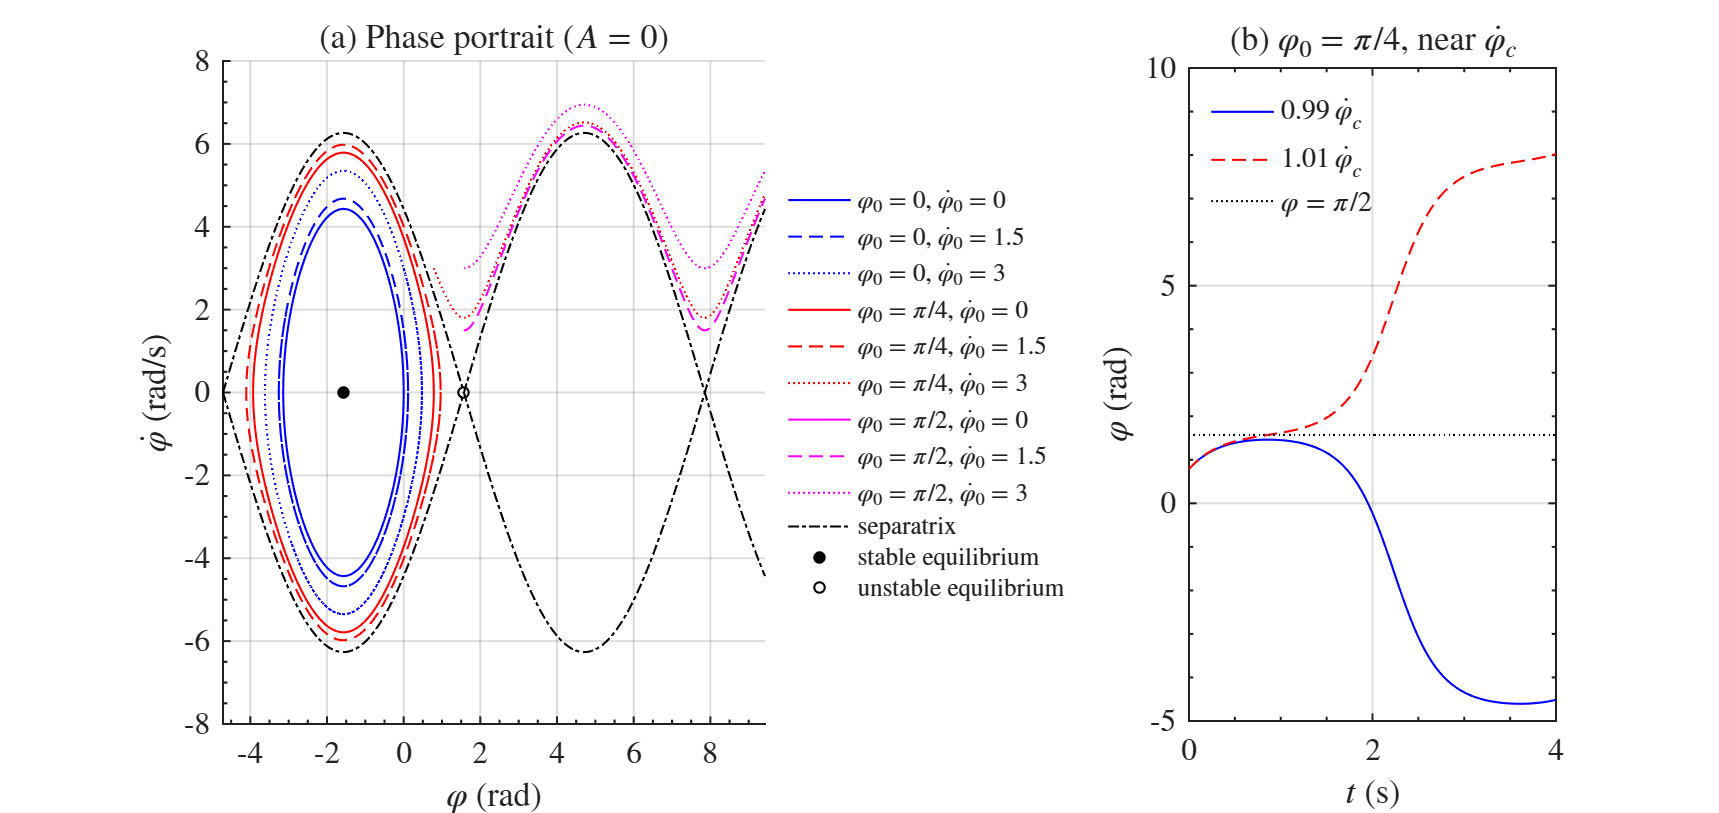
\includegraphics[width=0.84\textwidth]{Fig_5.png}
\caption{Fixed loop ($A=0$), item 7. (a) Phase portrait for the nine initial conditions, with the separatrix and the two equilibria. (b) $\varphi_0=\pi/4$ with $\dt\varphi_0$ 1\% below and above the critical rate of \cref{eq:crit}.}\label{fig:phase}
\end{figure}

\subsection{Linearized and full equation}
\Cref{fig:lin}a shows the percentage error $100\,|\delta_{\text{lin}}-\delta_{\text{full}}|/\max|\delta_{\text{full}}|$. It is divided by the amplitude of $\delta$ and not by $\delta$ itself, because $\delta$ crosses zero and the error relative to it would diverge there. The thick lines are the largest error reached up to each time. The \texttt{ode45} solution of \cref{eq:lin} matches the closed forms \cref{eq:linsol,eq:res} to \SI{2e-8}{rad}, so the differences come from the model and not from the integration. \Cref{tab:lin} gives the numbers.
\begin{table}[htbp]
\centering
\caption{Linearized against full equation, $t\in[0,10]$ s.}\label{tab:lin}
\begin{tabular}{lccc}
\toprule
$\omega$ & $\max|\delta_{\text{full}}|$ (rad) & error at $t=\SI{5}{s}$ & largest error\\
\midrule
$\sqrt{g/R}$ & 0.0134 & 6.68\% & 21.4\%\\
$\tfrac12\sqrt{g/R}$ & 0.196 & 3.30\% & 27.8\%\\
$\tfrac14\sqrt{g/R}$ & 0.0008 & 0.32\% & 1.86\%\\
\bottomrule
\end{tabular}
\end{table}

For $\omega=\sqrt{g/R}$, $\delta$ stays small but the error grows steadily up to 21\%. The reason is the term $\Omega^2\delta$ dropped in \cref{sec:lin}: it reduces the stiffness of the full equation from $g/R=\SI{981}{s^{-2}}$ by about $A^2\omega^2/2=\SI{4.9}{s^{-2}}$ on average, so the full solution oscillates about 0.25\% slower and falls behind the linear one. A frequency difference produces a phase lag that grows linearly with time, of about \SI{0.8}{rad} after \SI{10}{s}. For $\omega=\tfrac12\sqrt{g/R}$ the forcing frequency $2\omega$ equals $\omega_n$: this is the resonance of \cref{eq:res} \cite{notes}. Both solutions grow linearly (\cref{fig:lin}b) and reach \SI{0.196}{rad} ($11^\circ$) after \SI{10}{s}. The error stays small at first, but as $\delta$ grows, $\sin\delta\approx\delta$ stops being accurate and the full pendulum, whose period gets longer with the amplitude, slips out of step with the forcing; the error reaches 27.8\%. Without damping, the linear equation predicts unbounded growth, so for this $\omega$ the hypothesis $\delta\ll1$ always fails in the end. For $\omega=\tfrac14\sqrt{g/R}$ the forcing is far from resonance and 16 times weaker than in the first case: $\delta$ stays below \SI{8e-4}{rad}, the dropped term is negligible, and the error stays below 2\%. This is the case where the linearization works.

\begin{figure}[!htb]
\centering
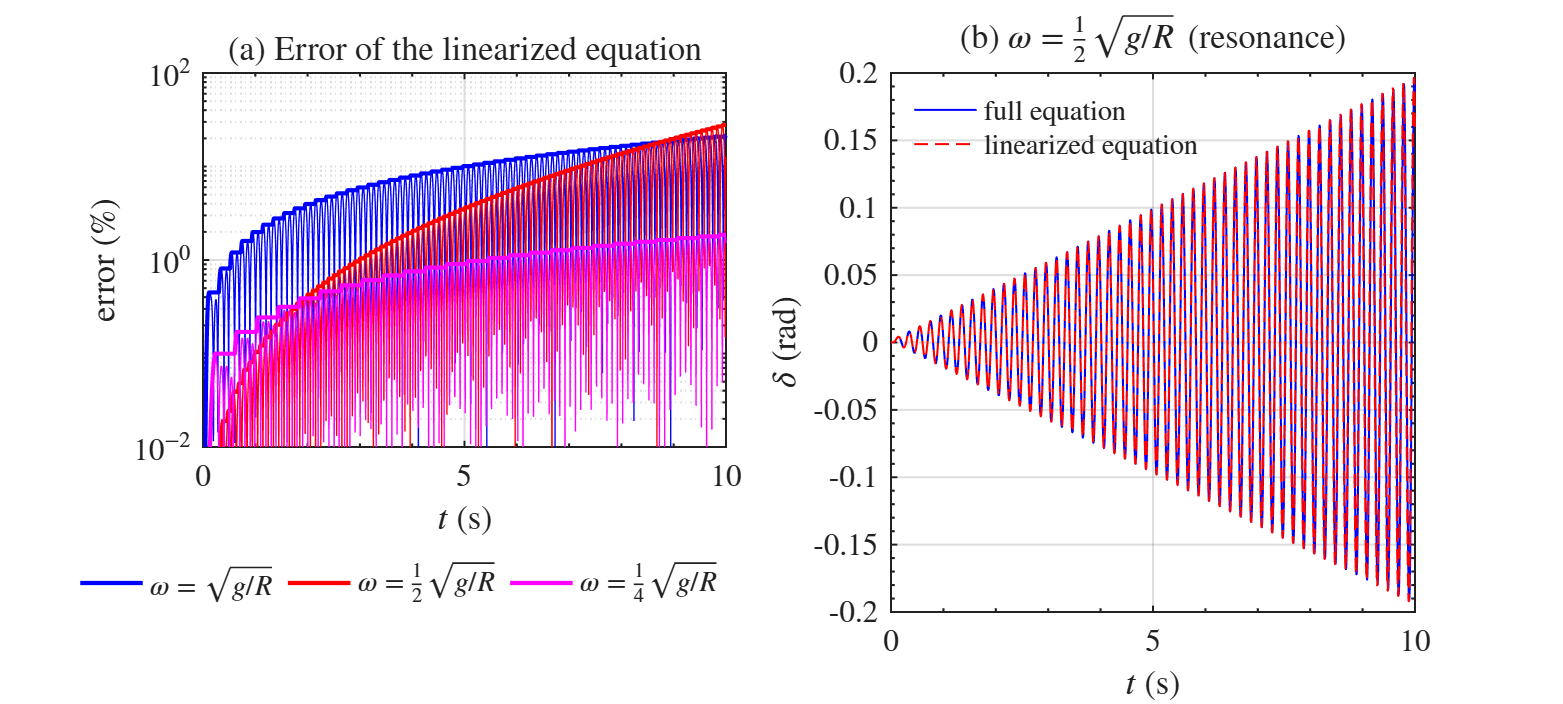
\includegraphics[width=0.82\textwidth]{Fig_6.png}
\caption{Item 8, $R=\SI{0.01}{m}$, $A=0.1$. (a) Percentage error of the linearized equation for the three frequencies; thin lines: error, thick lines: largest error up to each time. (b) Full and linearized solutions at resonance.}\label{fig:lin}
\end{figure}

%==============================================================
\section{Discussion}\label{sec:discussion}
Some points apply to the whole model and not to a single figure:
\begin{itemize}[noitemsep,topsep=2pt]
\item The equation of motion does not depend on $m$, and the rotation enters only through the centrifugal term. With $(A\omega)^2/(g/R)\approx1\%$, item 5 is close to a fixed pendulum; the rotation shows mostly in the reaction $N_z$ and in the energy.
\item The mechanical energy in the fixed frame is not conserved because the wire moves (\cref{eq:Edot}). In the rotating frame the reaction, the Euler force and the Coriolis force do no work, since they are normal to $\bm v_{\text{rel}}$, but the centrifugal potential $-\tfrac12m\Omega^2x^2$ depends on time, so $E_k^{\text{rel}}+E_p-\tfrac12m\Omega^2x^2$ is not conserved either. Only for constant $\Omega$, in particular $A=0$, is there a conserved energy, and the phase portrait of item 7 relies on it.
\item The seven checks of the code ($\ddt\varphi(0)$, $N_r=-3mg$, $E-E_0=W$, energy for $A=0$, distance to the axis, closed form of the linear solution and tolerances) test different parts of it, and all agree with \cref{sec:method}.
\item The results of item 8 depend on the initial conditions, which the statement does not give. With $\delta(0)\neq0$ a free oscillation of that amplitude would be added and the error would be divided by a larger $\max|\delta|$, but the two mechanisms, the phase lag and the resonance, would be the same.
\end{itemize}

%==============================================================
\section{Conclusions}\label{sec:conclusions}
The motion of a particle on a circular wire whose plane oscillates about a vertical axis was analysed in the rotating frame and integrated with \texttt{ode45}. The system has one degree of freedom, $\varphi$, and its equation contains only gravity and the centrifugal force. The Euler and Coriolis forces act normal to the plane and are balanced by the wire.

For the data of item 5 the rotation is slow and weak, so the particle swings like a pendulum of $90^\circ$ amplitude about the bottom with a period of \SI{2.37}{s}. The wire has to supply up to $3mg$ in its plane and up to \SI{2.78}{N} normal to it, almost all against the Coriolis force. The mechanical energy is not conserved because this normal reaction does work, but the work integrates back to almost zero every time the plane stops. Seen from a fixed frame, the particle draws a rosette of petals on the surface swept by the wire.

With the loop fixed, energy conservation gives the critical rate $\dt\varphi_c=\sqrt{(2g/R)(1-\sin\varphi_0)}$, and the nine initial conditions and the two cases at $\pm1\%$ of $\dt\varphi_c$ follow it. Finally, the linearized equation is a forced oscillator. It is accurate when the forcing is weak and far from resonance, it loses phase when the dropped term $\Omega^2\delta$ is not small enough, and it fails at resonance, $\omega=\tfrac12\sqrt{g/R}$, where the amplitude grows until $\delta\ll1$ no longer holds.

\begin{thebibliography}{9}
  \setlength{\itemsep}{1pt}
  \bibitem{guidelines}
  Aerospace Engineering Department (UC3M),
  \emph{Mechanics Applied to Aerospace Engineering: Laboratory Guidelines}, Version 2026.

  \bibitem{notes}
  Aerospace Engineering Department (UC3M),
  \emph{Mechanics Applied to Aerospace Engineering: course notes}, Sec.~5.4, ``Damped oscillator under a periodic force''.

  \bibitem{problems}
  Aerospace Engineering Department (UC3M),
  \emph{Mechanics Applied to Aerospace Engineering: particle exercises and problems}, Problem 34.

  \bibitem{matlab}
  The MathWorks, Inc.,
  \emph{MATLAB Documentation: ode45, odeset, VideoWriter, print}.
\end{thebibliography}

\end{document}
